% !TEX root = ../notes_unsupervisedlearning.tex
% Chapter 13: Reinforcement Learning Fundamentals
%%%%%%%%%%%%%%%%%%%%%%%%%%%%%%%%%%%%%%%%%%%%%%%%%%%%%%%%%%%%%%%%%%%%%%

\chapter{Reinforcement Learning Fundamentals}\index{Reinforcement Learning}\index{DQN}\index{PPO}
\newthought{Playing Atari.}

%══════════════════════════════════════════════════════════════════════
% BLOCK 1: INTRODUCTION
%═══════════════════════════════════════════════════════════════════════

\section{The Why}\index{reinforcement learning}\index{reward}\index{credit assignment}

\marginnote{\newthought{Reward.}\index{reward} A scalar number returned by the environment after an action,
carrying no information about which action would have been better, no gradient,
no class identity, only a magnitude and a sign. Let's extract signal yet again.}

\newthought{In the previous chapter} supervision still arrived as labels, 
but a label on a single input cannot transmit a sequence of decisions
or the consequences of one action on the next.
Reinforcement learning answers a complementary question:
What if the supervision is a scalar reward and depends on the sequence of actions a model takes?



\marginnote{\newthought{Simulation as substrate.}\index{simulation}\index{sim-to-real} 
Most reinforcement learning happens inside a simulator, 
since collecting millions of transitions on real hardware is prohibitive. 
The simulator's reward and transition function are perfect inside the sim and biased outside it, 
and the resulting sim-to-real gap is the central practical concern.}


\newthought{Markov decision processes.}\index{Markov Decision Process}
The setting is formalised~\cite{Bellman1961} as a tuple of a state $s$, an action $a$,
a transition probability $P(s' \mid s, a)$, a reward $r(s, a)$, and a discount factor $\gamma \in [0, 1)$.
The Markov property requires that the next state depends only on the current state and action,
which lets the agent reason forward without dragging the past along,
while $\gamma$ downweights rewards $t$ steps in the future by $\gamma^t$, keeping the sum of returns finite over infinite horizons.


\marginnote{\newthought{Pressure One: Credit assignment.}\index{credit assignment} The reward arrives 
long after the action that helped earned it. Bellman decomposition turns the long-horizon problem 
into a local fixed-point one.}

\newthought{Bellman equations.}\index{Bellman equation}
The value of a state under policy $\pi$ is the expected discounted return when starting in $s$ 
and following $\pi$ from then on.
Bellman's insight is that this value satisfies a local recursion:
The value of a state equals the expected immediate reward plus the discounted expected value of the next state.
This turns long-horizon optimisation into a fixed-point problem which suits Markovian dynamics.


\marginnote{\newthought{Model and policy.}\index{model}\index{policy} A model $\theta$ is the bag of parameters that 
gradient descent updates. A policy $\pi$ is the behaviour rule the agent acts under, mapping states to actions. 
The two coincide in policy-gradient methods, where $\theta$ directly parameterises $\pi_\theta$, 
but separate in value-based methods, where $\theta$ parameterises a value function $Q_\theta$ 
and the policy is derived from it as greedy or $\varepsilon$-greedy.}



\newthought{Value-based methods learn what each action is worth.}\index{Q-learning}\index{DQN}
A Q-learning agent maintains an action-value table and bootstraps each estimate against the next,
converging to the optimum even when behaviour is off-policy.
The Deep Q-Network, DQN, scales the table to a neural network for high-dimensional inputs,
which means a single set of weights now produces the value for every state-action pair,
and updating the weights for one state changes the values for all of them.
Two instabilities follow.

\newthought{Replay Buffer}\index{replay buffer}
First, the agent's experience is a stream of correlated transitions:
Each new state is the consequence of the previous one,
and the agent often spends long stretches in similar regions of the environment.
A network trained directly on this stream overfits to whatever region the agent is currently in
and forgets what it learned about earlier ones.
The experience replay buffer stores past transitions in a large pool
and samples minibatches uniformly from it,
so each gradient step sees a mix of transitions from many different points in time. Notice 
that this quickly becomes a compute bottleneck and does not scale.

\newthought{Target Network}\index{target network}
Second, the bootstrapped target uses the same network whose weights we are updating,
so each update changes both the predictions and the targets they are regressing against,
and convergence is unstable because the network is chasing a target that moves with it.
A target network is a slow-updating copy used only to compute that target,
kept frozen for thousands of steps so the online network has a stable regression problem
to converge to before the target shifts.

\marginnote{\newthought{Pressure Two: Stability.}\index{stability} Bootstrapped value estimates and policy gradients can amplify their own noise. Replay buffers, target networks, and trust regions stop the loop from running away.}

\newthought{Policy-based methods learn the action rule directly.}\index{policy gradient}\index{REINFORCE}\index{actor-critic}\index{advantage function}
A value-based method learns what each action is worth and then acts greedily,
deriving the policy from the value estimates.
A policy-based method skips the value function and parameterises a stochastic policy $\pi_\theta(a \mid s)$
that outputs the probability of each action directly. This also allows for continuous action spaces, 
where a value-based method regresses.
The policy gradient theorem turns the long-run expected return into a quantity we can backpropagate against,
and applies it by rolling out a trajectory, observing the return,
and nudging $\pi_\theta$ to make the actions that led to high return more likely
and those that led to low return less likely.

\marginnote{\newthought{Off-policy vs on-policy.}\index{off-policy}\index{on-policy} Q-learning and DQN learn from data collected under any behaviour, including a replay buffer of past transitions. Policy-gradient methods need data collected under the current policy, which is why trust regions matter: They control how far the new policy can drift before the old data stops applying.}

\newthought{Trust regions and clipping.}\index{PPO}\index{trust region}
Policy-gradient methods are on-policy: The gradient is computed under the old policy,
so if a single update moves the new policy too far the data no longer applies
and performance collapses.
Trust-region methods address this by explicitly constraining the size of the policy update,
which requires a second-order optimisation step that is expensive to compute. Proximal Policy Optimisation, PPO~\cite{Schulman2017PPO}, replaces the explicit constraint with a much simpler clipping trick.
Each action in a trajectory has a probability under the old policy and a probability under the new policy,
and their ratio measures how much the policy has shifted on that action since the last update.
PPO clips this ratio to a narrow band around one, typically $[0.8, 1.2]$,
before plugging it into the policy-gradient update.
The width of the band opts for stability over sample efficiency.
\marginnote{\newthought{Pressure Three: Exploration.}\index{exploration} Without enough variety in the data, the agent never sees the actions whose value it has yet to estimate. Exploration is the open subfield that supplies that variety.}

\newthought{Trade-off Exploration and Exploitation.}\index{exploration}\index{exploitation}
Every method above needs a behaviour rule for collecting data,
and that rule has to balance two pressures.
Exploit what is currently known to be good so reward is collected,
explore actions that are uncertain so the value estimates can improve.
$\varepsilon$-greedy, and entropy bonuses on the policyare the instruments that show up everywhere in practice,
and the design of better exploration is an open subfield in its own right.


\marginnote{\newthought{Atari and Go.}\index{Atari}\index{Go} A DQN agent learned to play forty-nine Atari games
from raw pixels and a single score signal~\cite{Mnih2015DQN}. The score arrives at the end of a life
or an episode, not after each frame, and the agent has to figure out by itself which of the thousands
of intermediate joystick presses earned it.}

\newthought{In order to move to learning from a scalar, model dependant reward} we have good reason to find ways to,
\begin{itemize}
    \item formalise sequential decision problems as Markov Decision Processes
    and decompose long-horizon value into a local Bellman recursion.
    \item learn action values by bootstrapping each estimate against the next,
    and stabilise the neural-network case with a replay buffer for decorrelated samples and a target network for a fixed regression target.
    \item parameterise a stochastic policy directly and update it by rolling out trajectories
    and reweighting actions according to the returns they led to.
    \item constrain how far each policy update is allowed to move from the previous one,
    so that the data collected under the old policy still informs the new one.
    \item collect informative experience under uncertainty,
    balancing exploitation of known reward against exploration of unfamiliar actions.
\end{itemize}

\newthought{The fundamental question} this chapter answers is whether a single scalar reward,
delayed and sparse, carries enough signal to teach an agent how to act,
without any teacher ever specifying what the right action would have been.

\newpage

\iffalse
\subsection{Hands On Experience}

\begin{marginfigure}
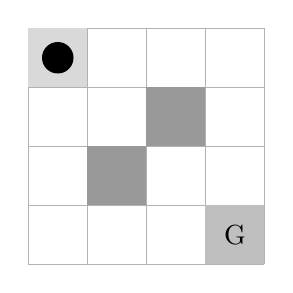
\begin{tikzpicture}[scale=0.5]
    % Grid
    \draw[step=1.5cm, black!30, thin] (0,0) grid (6,6);
    % Start
    \fill[black!15] (0,4.5) rectangle (1.5,6);
    \node at (0.75,5.25) {S};
    % Goal
    \fill[black!25] (4.5,0) rectangle (6,1.5);
    \node at (5.25,0.75) {G};
    % Obstacle
    \fill[black!40] (1.5,1.5) rectangle (3,3);
    \fill[black!40] (3,3) rectangle (4.5,4.5);
    % Agent
    \fill[black] (0.75,5.25) circle (0.4);
\end{tikzpicture}
\caption{Gridworld: navigate from S to G, avoiding obstacles.}
\label{fig:gridworld}
\end{marginfigure}

Consider a 4$\times$4 gridworld:
\begin{itemize}
    \item Start at top-left, goal at bottom-right
    \item Actions: up, down, left, right
    \item Reward: $+1$ at goal, $-1$ for hitting obstacle, $0$ otherwise
\end{itemize}

What is the optimal policy? How would you estimate the value of each state? What if you did not know the transition probabilities?

\newthought{The Learning Objectives} of this lecture:
\begin{itemize}
    \item Formalise problems as Markov Decision Processes, derive Bellman equations, and implement Q-learning by hand and with neural networks.
    \item Derive the policy gradient theorem, implement REINFORCE with a baseline, and explain the advantage function.
    \item Apply PPO for stable policy optimisation and compare value-based and policy-based methods for a given problem.
\end{itemize}

%═══════════════════════════════════════════════════════════════════════
% BLOCK 2: MAIN THEORY
%═══════════════════════════════════════════════════════════════════════

\newpage
\section{Markov Decision Processes}\index{Markov Decision Process}\index{MDP}

\marginnote{MDPs formalise sequential decision making under uncertainty.}

\newthought{A Markov Decision Process} is a tuple $(S, A, P, R, \gamma)$ where $S$ is the state space, $A$ is the action space, $P(s'|s,a)$ is the transition probability, $R(s,a,s')$ is the reward function, and $\gamma \in [0,1]$ is the discount factor.

\newthought{The Markov property:} the future depends only on the current state, not the history:
\begin{equation}
    P(s_{t+1} | s_t, a_t, s_{t-1}, a_{t-1}, \ldots) = P(s_{t+1} | s_t, a_t)
\end{equation}

\subsection{Policies and Value Functions}

\newthought{A policy}\index{policy} $\pi: S \to \Delta(A)$ maps states to action distributions.

\newthought{The state value function}\index{value function}:
\begin{equation}
    V^\pi(s) = \mathbb{E}_\pi \left[ \sum_{t=0}^\infty \gamma^t R_t \mid s_0 = s \right]
\end{equation}

\newthought{The action value function}\index{Q-function}:
\begin{equation}
    Q^\pi(s,a) = \mathbb{E}_\pi \left[ \sum_{t=0}^\infty \gamma^t R_t \mid s_0 = s, a_0 = a \right]
\end{equation}

\subsection{Bellman Equations}\index{Bellman equation}

\marginnote{Bellman equations: the foundation of RL algorithms.}

\begin{equation}
    V^\pi(s) = \sum_a \pi(a|s) \sum_{s'} P(s'|s,a) [R(s,a,s') + \gamma V^\pi(s')]
\end{equation}

\begin{equation}
    Q^\pi(s,a) = \sum_{s'} P(s'|s,a) [R(s,a,s') + \gamma \sum_{a'} \pi(a'|s') Q^\pi(s',a')]
\end{equation}

\newthought{The optimal} value function satisfies:
\begin{equation}
    Q^*(s,a) = \sum_{s'} P(s'|s,a) [R(s,a,s') + \gamma \max_{a'} Q^*(s',a')]
\end{equation}


\section{Value-Based Methods}\index{value-based methods}

\marginnote{Learn the Q-function, then act greedily.}

\subsection{Q-Learning}\index{Q-learning}

\newthought{Q-learning} updates Q-values toward the TD target~\cite{Watkins1992QLearning}:
\begin{equation}
    Q(s,a) \gets Q(s,a) + \alpha \left[ r + \gamma \max_{a'} Q(s',a') - Q(s,a) \right]
\end{equation}

\begin{algorithm}[H]
\caption{Q-Learning}
\begin{algorithmic}[1]
\State Initialize $Q(s,a)$ arbitrarily
\For{each episode}
    \State Initialize $s$
    \While{$s$ is not terminal}
        \State Choose $a$ using policy derived from $Q$ (e.g.\ $\varepsilon$-greedy)
        \State Take action $a$, observe $r$, $s'$
        \State $Q(s,a) \gets Q(s,a) + \alpha [r + \gamma \max_{a'} Q(s',a') - Q(s,a)]$
        \State $s \gets s'$
    \EndWhile
\EndFor
\end{algorithmic}
\end{algorithm}

\newthought{Properties:} Q-learning is off-policy, so it can learn from any behaviour policy. It is tabular, requiring an enumerable state-action space. Under mild conditions it converges to $Q^*$.


\section{Deep Q-Networks}\index{DQN}

\marginnote{\newthought{DQN.} Q-learning with neural network function approximation~\cite{Mnih2015DQN}.}

\newthought{For large or continuous state spaces,} use a neural network $Q_\theta(s,a)$:

\begin{equation}
    \mathcal{L}(\theta) = \mathbb{E}_{(s,a,r,s') \sim \mathcal{D}} \left[ (r + \gamma \max_{a'} Q_{\theta^-}(s',a') - Q_\theta(s,a))^2 \right]
\end{equation}

\newthought{Two key innovations} stabilise training:
\begin{enumerate}
    \item Experience replay\index{experience replay}: store transitions in buffer $\mathcal{D}$, sample randomly to break correlation
    \item Target network\index{target network}: use old parameters $\theta^-$ for the target, update periodically to prevent oscillation
\end{enumerate}

\begin{figure}
\centering
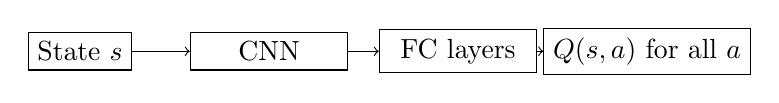
\begin{tikzpicture}[scale=0.8]
    \node[draw, rectangle] (state) at (0,0) {State $s$};
    \node[draw, rectangle, minimum width=2cm] (conv) at (3,0) {CNN};
    \node[draw, rectangle, minimum width=2cm] (fc) at (6,0) {FC layers};
    \node[draw, rectangle] (out) at (9,0) {$Q(s,a)$ for all $a$};

    \draw[->] (state) -- (conv);
    \draw[->] (conv) -- (fc);
    \draw[->] (fc) -- (out);
\end{tikzpicture}
\caption{DQN architecture: CNN processes pixels, outputs Q-value for each action.}
\label{fig:dqn}
\end{figure}


\section{Policy Gradient Methods}\index{policy gradient}

\marginnote{Directly optimise the policy, not the value function~\cite{Sutton1999PolicyGradient}.}

\subsection{Policy Parameterisation}

\newthought{The policy} $\pi_\theta(a|s)$ is a neural network outputting action probabilities. The objective is to maximise expected return:
\begin{equation}
    J(\theta) = \mathbb{E}_{\tau \sim \pi_\theta} \left[ \sum_t \gamma^t r_t \right]
\end{equation}

\subsection{Policy Gradient Theorem}

\begin{equation}
    \nabla_\theta J(\theta) = \mathbb{E}_{\pi_\theta} \left[ \nabla_\theta \log \pi_\theta(a|s) \cdot Q^{\pi_\theta}(s,a) \right]
\end{equation}

\subsection{REINFORCE}\index{REINFORCE}

\newthought{REINFORCE} uses a Monte Carlo estimate of $Q$~\cite{Williams1992REINFORCE}:

\begin{algorithm}[H]
\caption{REINFORCE}
\begin{algorithmic}[1]
\For{each episode}
    \State Generate trajectory $\tau = (s_0, a_0, r_0, \ldots)$ using $\pi_\theta$
    \For{each step $t$}
        \State $G_t \gets \sum_{k=t}^\infty \gamma^{k-t} r_k$ \Comment{Return from step $t$}
        \State $\theta \gets \theta + \alpha \gamma^t G_t \nabla_\theta \log \pi_\theta(a_t|s_t)$
    \EndFor
\EndFor
\end{algorithmic}
\end{algorithm}

\newthought{The problem:} high variance due to Monte Carlo estimation.

\subsection{Baseline Subtraction}\index{baseline}

\newthought{Reduce variance} by subtracting a baseline $b(s)$:
\begin{equation}
    \nabla_\theta J(\theta) = \mathbb{E} \left[ \nabla_\theta \log \pi_\theta(a|s) \cdot (Q(s,a) - b(s)) \right]
\end{equation}

Using $b(s) = V(s)$ gives the advantage\index{advantage function}: $A(s,a) = Q(s,a) - V(s)$.


\section{Actor-Critic Methods}\index{actor-critic}

\marginnote{Actor-Critic: combine policy gradient with value estimation.}

\newthought{The actor} is the policy $\pi_\theta(a|s)$ and the critic is the value function $V_\phi(s)$ or $Q_\phi(s,a)$. The critic estimates the advantage for actor updates:
\begin{equation}
    A(s,a) \approx r + \gamma V_\phi(s') - V_\phi(s)
\end{equation}

\subsection{Generalised Advantage Estimation}\index{GAE}

\marginnote{\newthought{GAE.} Balances bias and variance in advantage estimation~\cite{Schulman2016GAE}.}

\begin{equation}
    A_t^{\text{GAE}} = \sum_{l=0}^\infty (\gamma \lambda)^l \delta_{t+l}
\end{equation}

where $\delta_t = r_t + \gamma V(s_{t+1}) - V(s_t)$ is the TD error.


\section{Proximal Policy Optimization}\index{PPO}

\marginnote{\newthought{PPO.} Stable, sample-efficient, widely used~\cite{Schulman2017PPO}.}

\newthought{The problem with vanilla policy gradient:} large updates can destroy the policy.

\newthought{PPO's solution:} clip the objective to limit update size:

\begin{equation}
    \mathcal{L}^{\text{CLIP}}(\theta) = \mathbb{E} \left[ \min\left( r_t(\theta) A_t, \text{clip}(r_t(\theta), 1-\epsilon, 1+\epsilon) A_t \right) \right]
\end{equation}

where $r_t(\theta) = \frac{\pi_\theta(a_t|s_t)}{\pi_{\theta_{\text{old}}}(a_t|s_t)}$ is the probability ratio.

\begin{figure}
\centering
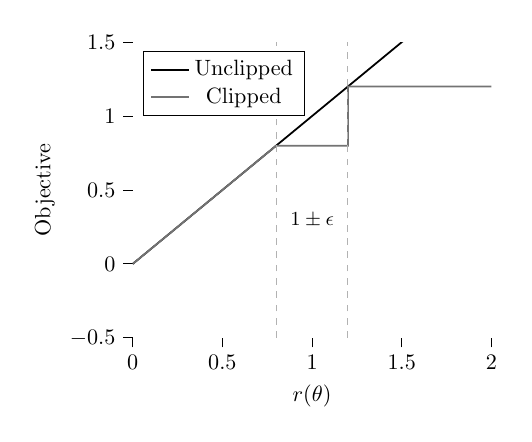
\begin{tikzpicture}[scale=0.8]
    \begin{axis}[
        xlabel={$r(\theta)$},
        ylabel={Objective},
        xmin=0, xmax=2,
        ymin=-0.5, ymax=1.5,
        width=0.6\textwidth,
        axis line style={draw=none},
        tick style={black, thin},
        tick align=outside, tick pos=left,
        legend pos=north west,
    ]
    % Unclipped (A > 0)
    \addplot[black, thick, domain=0:2] {x};
    % Clipped (A > 0)
    \addplot[black!55, thick] coordinates {
        (0,0) (0.8,0.8) (0.8,0.8) (1.2,0.8) (1.2,1.2) (2,1.2)
    };
    \draw[dashed, black!30] (axis cs:0.8,-0.5) -- (axis cs:0.8,1.5);
    \draw[dashed, black!30] (axis cs:1.2,-0.5) -- (axis cs:1.2,1.5);
    \node at (axis cs:1,0.3) {\small $1\pm\epsilon$};
    \legend{Unclipped, Clipped}
    \end{axis}
\end{tikzpicture}
\caption{PPO clipping: prevents too-large policy updates.}
\label{fig:ppo_clipping}
\end{figure}


%═══════════════════════════════════════════════════════════════════════
% BLOCK 3: STUDENT ACTIVATION
%═══════════════════════════════════════════════════════════════════════

\newpage
\section{Examples \& Exercises}

\subsection{Exercise 1: Q-Learning by Hand}

Gridworld: 3 states (A, B, C). A $\to$ B with $r{=}0$, B $\to$ C with $r{=}0$, C is terminal with $r{=}1$. $\gamma = 0.9$, $\alpha = 0.1$.

Initial $Q = 0$ everywhere. Update $Q(B, \text{right})$ after transition $B \to C$.

\subsection{Exercise 2: DQN Stability}

Why does DQN need both experience replay and target networks?

\subsection{Exercise 3: Policy Gradient Variance}

REINFORCE has high variance. Why does subtracting a baseline help?


\fi
\section{Self-Reflection and Recap}

\newthought{Self-Reflection} questions to guide your thinking:

\begin{itemize}
    \item Why does the Markov property let the agent reason about the future without dragging the past along, and what would change if the next state depended on the full history?
    \item Why does the discount factor $\gamma$ exist at all, and how does $\gamma < 1$ keep the sum of returns finite over infinite horizons?
    \item How does the Bellman recursion turn a long-horizon optimisation into a local fixed-point problem?
    \item What does it mean for Q-learning to be off-policy, and why does that property let DQN learn from a replay buffer of past transitions?
    \item Why does scaling the Q-table to a neural network introduce instabilities that the tabular case did not have, given that one set of weights now produces values for every state-action pair?
    \item What problem does the experience replay buffer solve, how does uniformly sampling past transitions from a large pool address it, and where does the approach run into a compute bottleneck?
    \item Why is a target network needed on top of the replay buffer, and what goes wrong when the target moves with the network being trained?
    \item How is a policy-based method different from a value-based method, why does parameterising $\pi_\theta(a \mid s)$ directly let you skip learning the value function, and how does this open the door to continuous action spaces?
    \item Why is the policy gradient theorem the key technical move that lets us treat the long-run expected return as a quantity we can backpropagate against?
    \item Why are trust regions and PPO clipping a policy-gradient concern only, and not relevant for Q-learning?
    \item Why does PPO clip the ratio between new and old policy probabilities to a narrow band such as $[0.8, 1.2]$, and how does the width of that band trade stability against sample efficiency?
    \item Why does every method in this chapter need a behaviour rule for exploration, and what role do $\varepsilon$-greedy, entropy bonuses on the policy, and stochastic policies play as the three blunt instruments?
\end{itemize}

\vspace{1.5em}

\newthought{Recap} of key concepts:

\begin{itemize}
    \item Markov decision processes formalise sequential decision making as the tuple $(s, a, P, r, \gamma)$ with the Markov property: the next state depends only on the current state and action, and $\gamma$ downweights rewards $t$ steps in the future by $\gamma^t$ to keep returns finite over infinite horizons.
    \item The Bellman equations decompose the value of a state into immediate reward plus discounted value of the next state, and almost every method in this chapter is a way to solve that local fixed-point problem under different practical constraints.
    \item Value-based methods learn what each action is worth and act greedily; Q-learning is off-policy and converges in the tabular case, and DQN scales it to neural networks with an experience replay buffer that mixes correlated transitions and a target network that holds the regression target still, though replay sampling becomes a compute bottleneck at scale.
    \item Policy-based methods skip the value function and parameterise a stochastic policy $\pi_\theta(a \mid s)$ directly, which also unlocks continuous action spaces where value-based regression struggles; the policy gradient theorem provides a backpropagatable surrogate, and PPO bounds the on-policy update by clipping the probability ratio between new and old policy to a narrow band around one.
    \item Exploration supplies the data variety the methods above consume; $\varepsilon$-greedy, entropy bonuses on the policy, and stochastic policies are the three blunt instruments, and better exploration is an open subfield in its own right.
\end{itemize}

\vspace{2.5em}

\marginnote{\newthought{Teaser.} Bellman decomposition makes long-horizon credit assignment tractable in principle. 
In practice, sparse rewards mean infeasible many steps before any informative signal arrives. 
What signal would shortcut all that?}

\newthought{Reinforcement learning's hardest problem is long-horizon credit assignment.}
Bellman decomposition reduces it to local updates,
but across sparse, long horizons it arrives too rarely to learn from on any practical budget.

\newthought{The next chapter turns to interactive and imitation learning,}
where we compress the long-horizon credit-assignment problem into a single demonstration,
correction, or preference.
Reinforcement learning derived its supervision from environmental reward;
interactive learning derives it from few-shot demonstrations, corrections, or preferences from an annotator.

\marginnote{\newthought{feedback}}
